\documentclass[11pt,letterpaper]{article}
\PassOptionsToPackage{hyphens}{url}
\usepackage[margin=.83in,top=.8in,bottom=.8in,headheight=15pt]{geometry}
\usepackage[T1]{fontenc}
\usepackage{lmodern,amsmath,amssymb,mathtools,bm,booktabs,array,graphicx,tikz}
\usetikzlibrary{arrows.meta,positioning,calc,decorations.pathreplacing,patterns}
\definecolor{ink}{HTML}{17344D}\definecolor{accent}{HTML}{087E8B}\definecolor{pale}{HTML}{EDF5F5}\definecolor{gold}{HTML}{AD6B19}
\providecommand{\dd}{\,\mathrm{d}}\providecommand{\R}{\mathbb{R}}
\providecommand{\E}{\mathbb{E}}\providecommand{\Var}{\operatorname{Var}}
\providecommand{\Cov}{\operatorname{Cov}}\providecommand{\diag}{\operatorname{diag}}
\providecommand{\norm}[1]{\left\lVert#1\right\rVert}
\providecommand{\abs}[1]{\left|#1\right|}
\usepackage{microtype,hyperref,fancyhdr,enumitem,amsthm,sectsty,needspace}
\allsectionsfont{\raggedright}
\hypersetup{colorlinks=true,linkcolor=ink,urlcolor=accent,pdfauthor={Zan Ahmad},pdftitle={Shape comparisons, deformation penalties and geometric matching / Lecture notes}}
\setlength{\parindent}{0pt}\setlength{\parskip}{6pt}\linespread{1.07}
\setlist{itemsep=3pt,topsep=4pt,leftmargin=*}
\emergencystretch=2em\clubpenalty=10000\widowpenalty=10000
\pagestyle{fancy}\fancyhf{}\fancyhead[L]{\small Computational Cardiology}\fancyhead[R]{\small Lecture 14}
\fancyfoot[L]{\footnotesize Zan Ahmad}\fancyfoot[R]{\footnotesize\thepage}\renewcommand{\headrulewidth}{.3pt}
\newtheorem{proposition}{Proposition}\newtheorem{theorem}{Theorem}\newtheorem{lemma}{Lemma}
\theoremstyle{definition}\newtheorem{definition}{Definition}\newtheorem{example}{Example}
\numberwithin{equation}{section}
\begin{document}
{\small\scshape Computational Cardiology\hfill Lecture 14}\par\medskip
{\raggedright\hyphenpenalty=10000\exhyphenpenalty=10000\LARGE\bfseries\color{ink} Shape comparisons, deformation penalties and geometric matching\par}\medskip
{\small Lecture notes}\par\bigskip
Rigid alignment and cyclic indexing remove selected nuisance transformations from a contour comparison. A deformation penalty then distinguishes displacement patterns with equal RMS amplitude. These finite calculations provide a mathematical bridge to elastic path energies and varifold endpoint terms without claiming to implement those research methods.

\section{A finite cohort and its comparison rule}
\hypertarget{note-a-finite-cohort-and-its-comparison-rule}{}\label{note:a-finite-cohort-and-its-comparison-rule}
{\small \href{slides.html\#frame=a-comparison-requires-an-invariance-choice\&step=1}{Slides for this section} \quad \href{../modules/shape-lab/index.html}{Landmark geometry and ambient flows} \quad \href{../modules/animations/landmark-flow.html}{Correspondence, interpolation and flow}}\par
Before comparing a cohort, state which differences should count. If coordinate origin and orientation are arbitrary, raw coordinate RMS measures a mixture of pose and geometry. If physical size matters, normalizing every contour to unit size would remove part of the scientific signal. A distance therefore has no interpretation independent of representation, correspondence, units and allowed transformations. These choices should be recorded before examining which subjects appear close or far apart.

Our cohort contains five original synthetic contours sampled at 64 ordered points. A is a reference. B is a rotated and translated copy. C is 15 percent larger. D has a smooth local displacement in the positive x direction over a short region. E is the same stored contour as A with a different cyclic starting index. None is a patient surface or a clinical morphology class. The deliberate construction gives known relationships against which the computation can be checked.

The first matrix uses raw fixed-index RMS in millimetres. It can place B or E far from A even though their underlying stored geometry is unchanged by the prescribed operations. The second matrix minimizes over proper rigid motions and all 64 cyclic starting shifts. That rule should identify A, B and E up to roundoff, while retaining size and local geometric differences. Comparing the two matrices reveals how a nuisance choice can dominate a result before any clustering method is applied.

The cohort is constructed so that some differences are known in advance: a rigid copy and a cyclic reindexing should agree with the reference under the declared quotient, while scaling and local displacement remain visible. This construction separates the definition of the comparison from any subsequent clustering algorithm.
\section{Cyclic rigid alignment}
\hypertarget{note-cyclic-rigid-alignment}{}\label{note:cyclic-rigid-alignment}
{\small \href{slides.html\#frame=cyclic-rigid-discrepancy\&step=1}{Slides for this section} \quad \href{../modules/shape-lab/index.html}{Landmark geometry and ambient flows} \quad \href{../modules/animations/landmark-flow.html}{Correspondence, interpolation and flow}}\par
A closed boundary has no necessary first vertex. If traversal direction is fixed, shifting every index by the same integer simply chooses a different start. The companion enumerates each possible shift, performs a proper rigid fit for that pairing, and retains the smallest RMS. Enumeration is feasible for this small teaching dataset and makes the search explicit. It preserves the ordering and direction of points; it does not permit a local stretch of one boundary region relative to another.

The minimized RMS cannot exceed the raw RMS because the identity shift, identity rotation and zero translation are among the permitted choices. The matrix is symmetric to numerical precision and has a zero diagonal. These are useful implementation checks. They do not guarantee that the comparison encodes the intended anatomy. Reflection, orientation reversal, arbitrary reparametrization and scale normalization remain excluded. Changing one of those choices requires a new name and explanation for the resulting comparison.

For this finite synthetic cohort, A--B and A--E aligned discrepancies are below 10 to the minus twelve millimetres. A--C is approximately 1.567 mm and A--D approximately 0.684 mm. Those are computed properties of the construction and the chosen fit. The matrix plots use separately labeled color scales so the smaller aligned differences remain visible. Compare printed values and units across panels; equal shades in panels with different scales do not imply equal distances.

\[
d_{\rm rc}(X,Y)=\min_{k,R,t}\sqrt{\frac1n\sum_j\|x_j-(y_{j+k}R+t)\|^2}
\]
Indices wrap modulo n. Coordinates, translation and distance are in mm. R is orthogonal with determinant +1; no scale factor or reversal is searched.

For a shift $k$, let $S_kY$ be the cyclically permuted array. Compute the proper Procrustes fit for each $k$ and take the minimum. There are $n$ candidate shifts, and the identity candidate is included, so
\[
 d_{rc}(X,Y)\le d_{\rm RMS}(X,Y).
\]
The search preserves ordering and traversal direction. Local reparametrization and reversal are different operations and are not introduced by enumerating cyclic starts.
\begin{center}\begin{minipage}{.98\linewidth}\centering
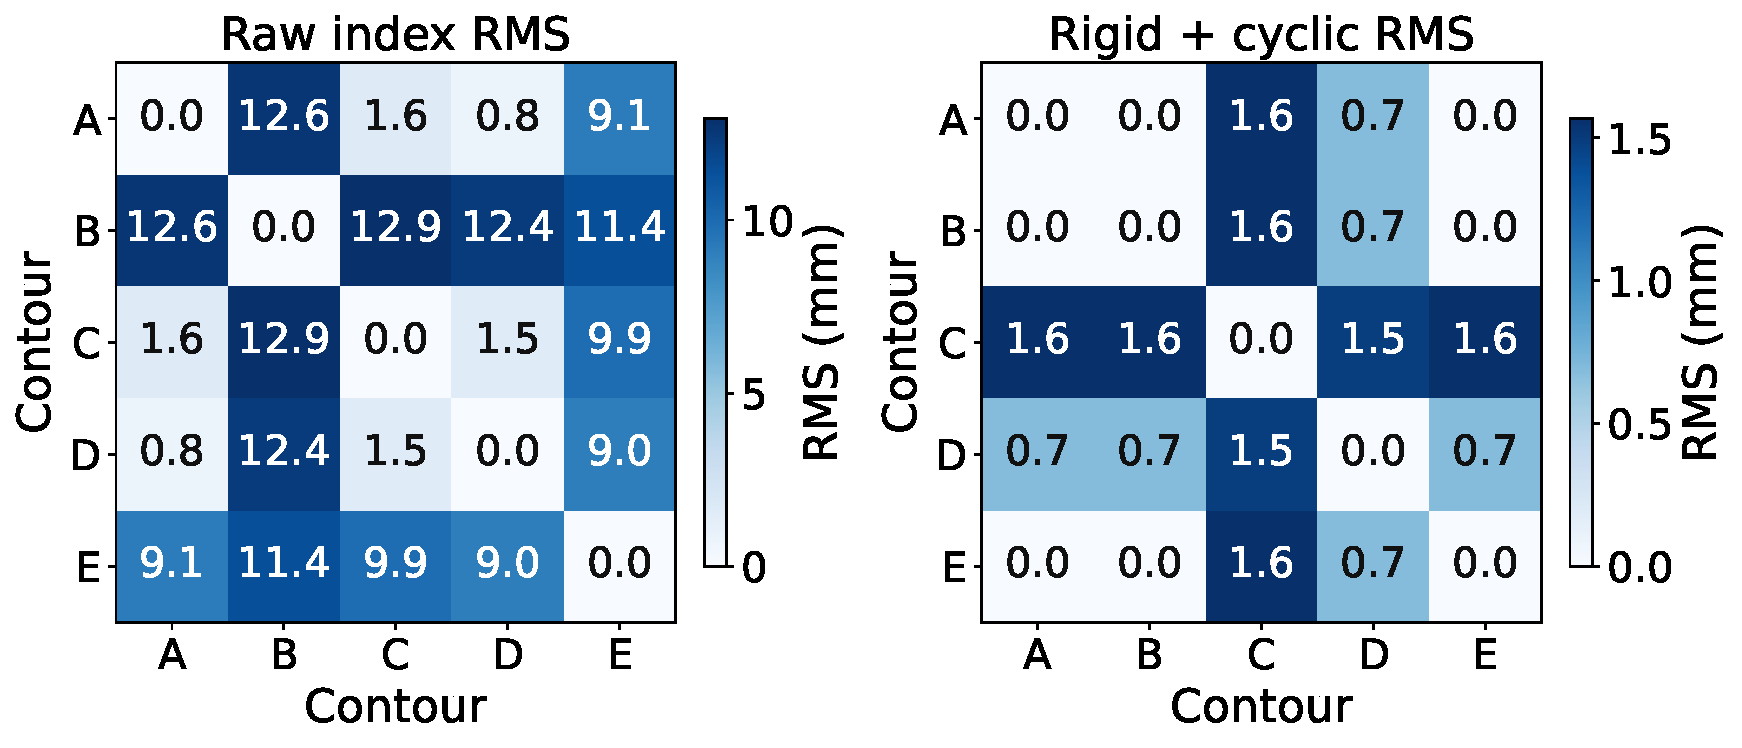
\includegraphics[width=.96\linewidth,height=.57\textheight,keepaspectratio]{cohort-distances.pdf}\par\smallskip
{\small Original 64-point synthetic contours: A reference; B posed copy; C 15\% larger; D local bulge; E cyclic index shift. Raw RMS includes pose and start artifacts. Proper rigid plus cyclic minimization removes those specified effects while preserving size/local differences. The panels have separate color scales in mm; read numeric entries across panels.}
\end{minipage}\end{center}
\section{Amplitude and neighbor-variation penalties}
\hypertarget{note-amplitude-and-neighbor-variation-penalties}{}\label{note:amplitude-and-neighbor-variation-penalties}
{\small \href{slides.html\#frame=equal-rms-does-not-imply-equal-displacement-pattern\&step=1}{Slides for this section} \quad \href{../modules/shape-lab/index.html}{Landmark geometry and ambient flows}}\par
A coordinate discrepancy treats each paired displacement as a vector. Its average squared length records amplitude, but it ignores how those displacements vary from one neighbor to the next. A broad, smooth deformation and a rapidly alternating one can therefore have the same RMS amplitude. If the application regards these patterns differently, a richer comparison must introduce additional structure and justify its weighting.

To make that idea hand-computable, define a finite score on a fixed cyclic list of displacement vectors. The first term is the mean squared displacement. The second is the mean squared difference between neighboring displacement vectors, multiplied by a nonnegative weight. The closing neighbor pair is included. With displacements in millimetres, both terms have units mm\ensuremath{^{2}} and the weight is dimensionless. This is a teaching score on a declared grid, not a physical energy in joules.

The roughness term vanishes for a constant displacement field, but the amplitude term still penalizes that translation. Thus the score does not automatically remove pose. It is applied here to supplied displacement patterns after the comparison question has been fixed. Changing the number or spacing of grid points changes the meaning of neighbor differences; this formula has no arclength derivative normalization. A continuum deformation model would require a suitable discretization and its own refinement analysis.

\[
E_\lambda(u)=\frac1n\sum_j\|u_j\|^2+\lambda\frac1n\sum_j\|u_{j+1}-u_j\|^2,\qquad\lambda\ge0
\]
u is a fixed cyclic array in mm; E has units mm\ensuremath{^{2}}. The nonnegative dimensionless weight changes the penalty for roughness. No path or correspondence is optimized.

Let $(Du)_j=u_{j+1}-u_j$ on the cycle. The score can be written
\[
 E_\lambda(u)=\frac1n u^{\mathsf T}(I+\lambda D^{\mathsf T}D)u.
\]
For vector displacements the same expression is summed over coordinate components. Since $I+\lambda D^{\mathsf T}D$ is positive definite for $\lambda\ge0$, $\sqrt{E_\lambda}$ is a norm on the fixed displacement array. That fact does not identify it with a distance between unparametrized surfaces.

\paragraph{Calculation.} A six-point cyclic field has scalar x displacements [1,1,1,\ensuremath{-}1,\ensuremath{-}1,\ensuremath{-}1] mm and zero y components. Compare with [1,\ensuremath{-}1,1,\ensuremath{-}1,1,\ensuremath{-}1] mm. Use weight 0.25.

Each field has mean squared amplitude 1 mm\ensuremath{^{2}}.

The first has two jumps of magnitude 2 mm, giving roughness 8/6 = 4/3 mm\ensuremath{^{2}}.

The second has six such jumps, giving roughness 24/6 = 4 mm\ensuremath{^{2}}.

Scores are 1 + 0.25\ensuremath{\times}4/3 = 4/3 mm\ensuremath{^{2}} and 1 + 0.25\ensuremath{\times}4 = 2 mm\ensuremath{^{2}}.

Equal RMS amplitudes need not give equal scores when neighbor variation is weighted.
\section{Fourier interpretation of the roughness weight}
\hypertarget{note-fourier-interpretation-of-the-roughness-weight}{}\label{note:fourier-interpretation-of-the-roughness-weight}
{\small \href{slides.html\#frame=scaling-and-constant-shifts\&step=1}{Slides for this section} \quad \href{../modules/shape-lab/index.html}{Landmark geometry and ambient flows}}\par
The second figure supplies two displacement fields on a fixed 64-point ring. One varies slowly around the ring; the other oscillates more rapidly. Both are normalized to RMS amplitude 1 mm and have mean displacement approximately zero. Their amplitude terms therefore agree. The computed neighbor terms are approximately 0.0479 and 0.8942 mm\ensuremath{^{2}}, so increasing the nonnegative weight raises the oscillatory score faster. At weight zero the scores tie exactly apart from roundoff.

This comparison isolates a mathematical preference, not an observation that one pattern is more biologically plausible. The chosen weight expresses how much the declared score penalizes neighbor variation. Multiplying all displacements by two multiplies both terms and the score by four. A zero field gives zero score, and adding a constant vector changes the amplitude term while leaving neighbor differences unchanged. These limits make good tests because their expected outcomes follow directly from the definition.

Keep the distinction between a score and a distance clear. The displayed quadratic value has squared-length units and is not presented as a metric. Its square root defines a weighted norm on these fixed displacement arrays when the weight is nonnegative, but that fact alone does not create an elastic distance between unparametrized shapes. Such a claim would require defining the shape space, admissible paths, invariances and optimization, then verifying the implementation. The supplied program performs none of that path search.

With Fourier coefficients $\widehat u_k=n^{-1}\sum_j u_j e^{-2\pi\mathrm i jk/n}$, Parseval's identity gives
\[
 E_\lambda(u)=\sum_{k=0}^{n-1}
 \left[1+4\lambda\sin^2(\pi k/n)\right]\|\widehat u_k\|^2.
\]
The constant mode has no neighbor penalty. Higher-frequency modes receive larger weights, reaching $1+4\lambda$ at the alternating mode on an even grid. Because $D$ is an unnormalized neighbor difference, changing sample spacing changes the continuum interpretation of this score.
\begin{center}\begin{minipage}{.98\linewidth}\centering
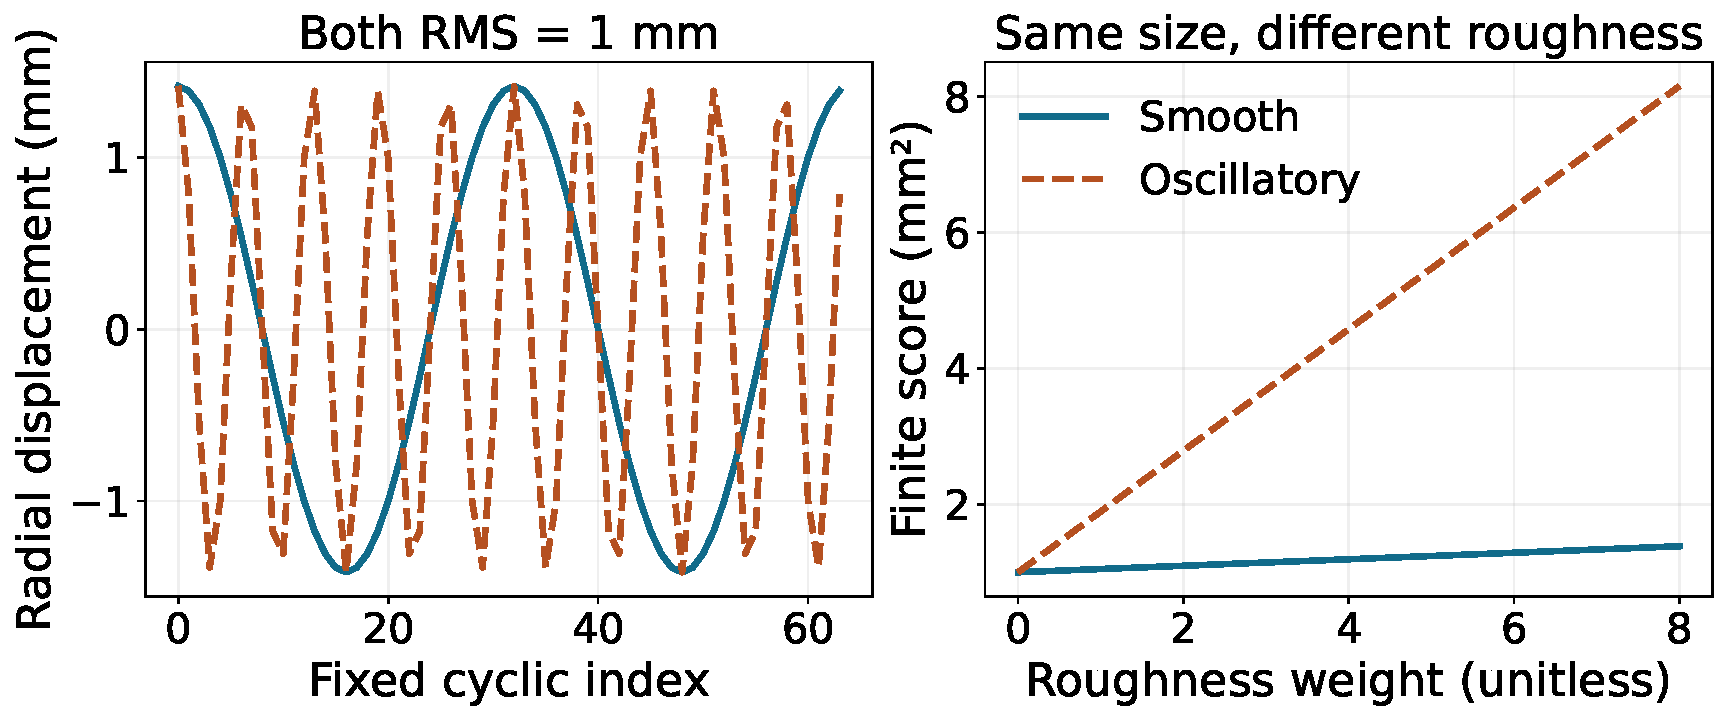
\includegraphics[width=.96\linewidth,height=.57\textheight,keepaspectratio]{displacement-cost.pdf}\par\smallskip
{\small Two supplied zero-mean displacement fields on a fixed 64-point ring both have RMS amplitude 1 mm. Their mean squared neighbor differences are about 0.0479 and 0.8942 mm$^2$. The finite score grows linearly with the nonnegative weight, illustrating a declared penalty preference rather than a full elastic shape distance.}
\end{minipage}\end{center}
\section{Elastic path energy and varifold endpoints}
\hypertarget{note-elastic-path-energy-and-varifold-endpoints}{}\label{note:elastic-path-energy-and-varifold-endpoints}
{\small \href{slides.html\#frame=elastic-energy-along-a-path\&step=1}{Slides for this section} \quad \href{../modules/shape-lab/index.html}{Landmark geometry and ambient flows} \quad \href{../modules/animations/landmark-flow.html}{Correspondence, interpolation and flow}}\par
The later published appendage paper considers three-dimensional surfaces and an elastic geometric framework. Its methods define a second-order Sobolev metric with weights controlling different deformation contributions, and compare surfaces through paths. The relaxed numerical matching problem combines a path-energy term with an endpoint-discrepancy term. These are distinct roles: the path term evaluates deformation along the route, while the endpoint term penalizes failure to match the target. The reported approximate elastic distance uses the optimized path energy, rather than silently treating the entire penalized objective as the distance.

Our finite example illustrates only the idea that weighting different deformation patterns changes a comparison. It has no surface differential operators, time-discretized path, endpoint optimizer or quotient over general reparametrizations. The 2025 reference paper supplies the broader mathematical context. This finite example does not use its patient data.

A complementary geometric representation represents local geometry through positions and tangent information with geometric weights. Nonoriented varifolds treat opposite tangent orientations as equivalent, and support comparison without a prescribed vertex-to-vertex pairing. The Charon--Trouvé reference develops this representation. Its kernel choices and spatial scale affect what discrepancies are emphasized. A varifold endpoint term still needs a separately specified deformation model if it is used to drive registration. This lesson implements no varifold distance or registration routine; deriving and validating one belongs to an extension.

Schematically, elastic matching minimizes a path functional such as
\[
 \int_0^1 G_{c(t)}(\dot c(t),\dot c(t))\,\mathrm dt
 +\gamma\|\mu_{c(1)}-\mu_{target}\|_K^2.
\]
The first term measures deformation along a path; the second penalizes an endpoint mismatch. In a nonoriented geometric representation, a kernel may use squared tangent or normal dot products so that opposite orientations give the same value. The positions, geometric weights and kernel scale all affect the endpoint discrepancy. This schematic expression explains the two roles; the companion computes neither a path optimizer nor a varifold norm. The later 2025 appendage paper uses a second-order Sobolev surface framework and reports path-energy-based approximate distances, not the entire penalized objective as an elastic distance.
\section{Invariant comparisons and scientific interpretation}
\hypertarget{note-invariant-comparisons-and-scientific-interpretation}{}\label{note:invariant-comparisons-and-scientific-interpretation}
{\small \href{slides.html\#frame=the-implemented-and-contextual-calculations\&step=1}{Slides for this section} \quad \href{../modules/shape-lab/index.html}{Landmark geometry and ambient flows} \quad \href{../modules/animations/landmark-flow.html}{Correspondence, interpolation and flow}}\par
A clustering algorithm can divide any such finite collection, but a partition does not create biological categories. Our A, B and E copies were constructed to agree; grouping them is an implementation check rather than a discovery. Five invented contours cannot validate a clinical classifier, stroke-risk relationship or population morphology distribution. Any grouping consequently depends on the imposed nuisance transformations and retained size or local differences.

A partition of the synthetic distance matrix reflects the chosen invariances and constructed examples. It is not evidence for clinical morphology classes. In particular, removing physical scale before comparison would erase a distinction deliberately retained here. The interpretable result is a comparison under a declared representation and transformation group, with sampling and deformation sensitivity still visible.
\bigskip
\section*{Exercises}
\par\noindent\begin{minipage}{\linewidth}
\subsection*{A14-1. Find a starting-index artifact}
X =\allowbreak{} [(0,0),(2,0),(2,1),(0,1)] mm. Y =\allowbreak{} [(2,0),(2,1),(0,1),(0,0)] mm. New formative practice; 10 feedback points.

\textbf{a} Calculate raw fixed-index RMS.

\end{minipage}\par\medskip
\textbf{b} Give the cyclic roll of Y that exactly recovers X and the minimized RMS.

\textbf{c} Explain why this result does not establish invariance to arbitrary local reparametrization.

\par\noindent\begin{minipage}{\linewidth}
\subsection*{A14-2. Compute a finite deformation score}
For four cyclic points, compare u =\allowbreak{} [(1,0),(0,1),(-1,0),(0,-1)] mm and v =\allowbreak{} [(1,0),(-1,0),(1,0),(-1,0)] mm. New practice; 10 feedback points.

\textbf{a} Compute the mean squared amplitude and mean squared neighbor difference of each field, including the closing pair.

\end{minipage}\par\medskip
\textbf{b} Find both scores at weight 0.5 and at weight zero, with units.

\textbf{c} Explain why these values are neither mechanical energies in joules nor outputs of an elastic path optimization.

\par\noindent\begin{minipage}{\linewidth}
\subsection*{A14-3. Check the limits of a score}
For any nonzero cyclic field u, let A be its amplitude term and B its roughness term. Assume a nonnegative weight. New practice; 10 feedback points.

\textbf{a} Derive the score for 3u and compare it with that for u.

\end{minipage}\par\medskip
\textbf{b} For a constant displacement u\_j =\allowbreak{} (2,-1) mm at every point, compute A, B and the score for any allowed weight.

\textbf{c} Can you change point count and interpret the same weight as an unchanged continuum roughness penalty? Explain what is missing.

\par\noindent\begin{minipage}{\linewidth}
\subsection*{A14-4. Audit a morphology claim}
A report clusters five synthetic contours using the raw matrix, calls the clusters clinical morphologies, and labels the implemented finite score an elastic distance. New practice; 10 feedback points.

\textbf{a} Identify an alignment artifact to check and give its predicted behavior under the lesson's corrected comparison.

\end{minipage}\par\medskip
\textbf{b} State two missing mathematical components required before claiming to implement the paper's full elastic method.

\textbf{c} Rewrite the clinical claim with a supported scope and name evidence needed for a clinical conclusion.

\section*{References}
\noindent\begin{minipage}{\linewidth}
Zan Ahmad, Advanced Topics in Computational Cardiology syllabus, Fall 2024. PDF pages 1--2.

\end{minipage}\par\medskip
\noindent\begin{minipage}{\linewidth}
Ahmad et al., A computational pipeline for clustering left atrial appendage morphology via elastic shape analysis, Computers in Biology and Medicine 196 (2025), 110905. PDF pages 2--4, methods: geometric representation, elastic path energy and relaxed matching.

\end{minipage}\par\medskip
\noindent\begin{minipage}{\linewidth}
Charon and Trouvé, The varifold representation of non-oriented shapes for diffeomorphic registration (2013). PDF page 1 abstract; PDF pages 8--10, end of section 3.1, section 3.2 and beginning of section 4: nonoriented tangent representation, discrete approximation and kernel-metric motivation.

\url{https://arxiv.org/abs/1304.6108}
\end{minipage}\par\medskip
\end{document}
